\documentclass[11pt, oneside]{article}   	% use "amsart" instead of "article" for AMSLaTeX format
\usepackage{geometry}                		% See geometry.pdf to learn the layout options. There are lots.
\geometry{letterpaper}                   		% ... or a4paper or a5paper or ... 
\usepackage{graphicx}				% Use pdf, png, jpg, or eps§ with pdflatex; use eps in DVI mode
								% TeX will automatically convert eps --> pdf in pdflatex		
\usepackage{amssymb}
\usepackage{amsmath}
\usepackage{parskip}
\usepackage{color}
\usepackage{hyperref}

\graphicspath{{/Users/telliott_admin/Tex/png/}}
% \begin{center} 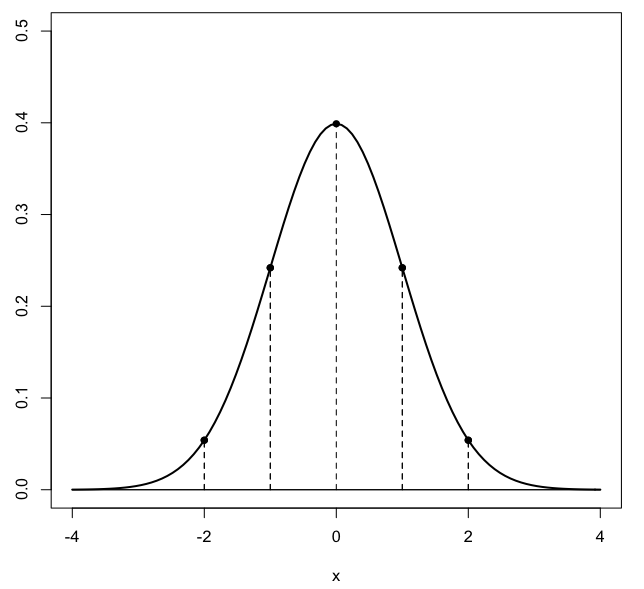
\includegraphics [scale=0.4] {gauss3.png} \end{center}

%break
\title{Pappus}
\date{}

\begin{document}
\maketitle
\Large

\label{sec:Pappus}

Pappus' centroid theorem is actually a pair of theorems about solids of revolution, where a curve $C$ is revolved around a central axis.  The two theorems relate to the surface area and volume.  

There is a nice article about it at Mathworld:

\url{http://mathworld.wolfram.com/PappussCentroidTheorem.html}

\section*{Area}

The first theorem states that the surface area $A$ is the product of the arc length $s$ of the curve $C$ times the distance $d$ traveled by the geometric centroid of $C$.
 
The example in the wikipedia article is a torus of minor radius $r$ and major radius $R$.  Then $C$ is a circle of radius $r$, the centroid of the curve is its center, and this point moves around a circle of radius $R$ the distance $2\pi R$.  

The first term is the circumference $C$ of the curve (the small circle) and the total is
\[ A = 2 \pi r \ 2 \pi R = 4 \pi^2 r R \]

One puzzling thing is that we are used to taking account of the slant height in thinking about surface area (though not volume), but the curvature of the surface doesn't seem to be an issue here.

\subsection*{Cylinder}
Here is a picture from Wolfram.  Our notation is slightly different.
\begin{center} 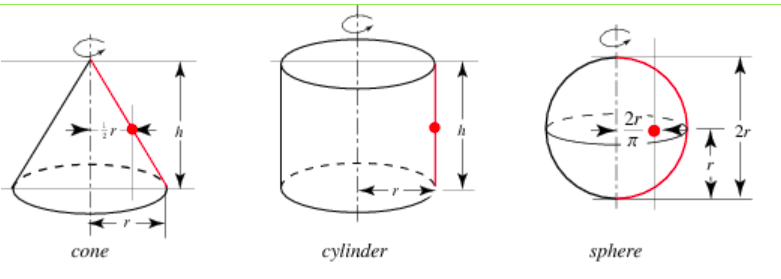
\includegraphics [scale=0.5] {pappus1.png} \end{center}

The cylinder is our first example, and here it's easy.  We revolve a parallel line segment around the $y$-axis.  The curve has length $H$. 

The centroid of the parallel line segment (the average distance of each point on the curve from the $y$-axis) is just the radial distance R, since all the points are the same distance away.  In addition, the centroid is also halfway along the curve at $H/2$.  

The distance it travels is $2\pi R$.

The surface area is the product of the arc length $H$ and the distance traveled by the centroid during the revolution

\[A = H 2 \pi R \]

The classical way to obtain a formula for the surface area of the cylinder is to imagine cutting along the length of it, forming a rectangle with width $H$ and length $2 \pi R$.  This gives the same result.

\subsection*{Cone}

For the cone, we revolve an inclined line segment around the $y$-axis, with one end on the axis and the other at the radius $R$.  The centroid of this line segment lies at a distance $R/2$ from the $y$-axis.  

The distance it travels during the rotation is then $\pi R$.

The length of the curve is the slant height $s$.  Multiplying to get the surface area

\[ A = \pi R s \]

The classical way to obtain this formula for the surface area of a cone (which we saw in a previous chapter) is to imagine cutting along the slant of the cone to obtain a sector of a circle.  The circle has radius $s$ and circumference $2 \pi s$ and area $\pi s^2$.  We take the ratio of the outer perimeter of the sector to the whole circumference, times the whole area

\[ \frac{2 \pi R}{2 \pi s} \ \pi s^2 = \pi R s \]

\subsection*{Sphere}

For the sphere, we revolve a half-circle around the $y$-axis.  Going back to the Mathworld article, we see that the centroid for the curve is

\[ \bar{x} = \frac{2 R}{\pi} \] 

and the centroid for the whole area of the semi-circle is

\[ \bar{x} = \frac{4 R}{3 \pi} \]

I will show how to derive these below.  To find the surface area of our solid of revolution (the sphere), we need to multiply the distance traveled by the centroid of the curve, $2 \pi \bar{x}$, times the length of the curve, $\pi R$
\[ A = 2 \pi \ \frac{2 R}{\pi} \ \pi R = 4 \pi R^2 \]

\section*{Volume}
The second theorem depends on the area enclosed by the curve (and the $y$-axis).  

The volume of the solid is the product of this area times the distance d traveled by the geometric centroid of the area (not the curve).  For the torus or donut
\[ V = \pi r^2 \ 2 \pi R = 2 \pi^2 R r^2 \]
 
Part of the trick here is going to be actually finding the geometric centroids.  
\subsection*{Cylinder}
\begin{center} 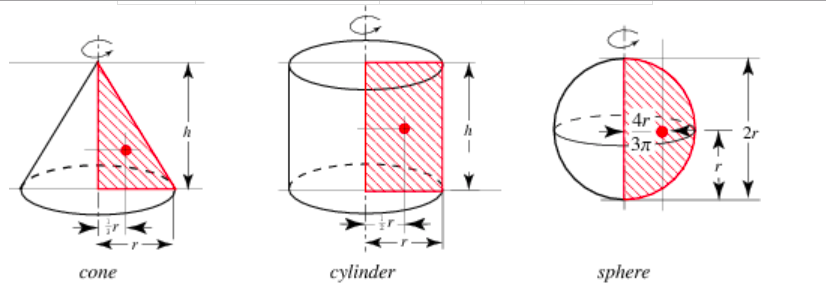
\includegraphics [scale=0.5] {pappus2.png} \end{center}

To find the volume of the cylinder, we need to consider the area enclosed by the curve and the $y$-axis (called a lamina).  

For the cylinder, the centroid of the lamina is at $R/2$ and its area is $RH$.  Multiply the area times the distance traveled by the centroid
\[ V = R H \ 2 \pi \frac{R}{2} = \pi HR^2  \]

\subsection*{Cone}

For the volume of the cone, we need to look at the triangle formed from the inclined line segment.  Its area is $Rh/2$.  Now, what is its geometric centroid?  

To begin with, I will just use the available result from wikipedia, which is that the centroid of a right triangle is $1/3$ of the distance along each side away from the right angle, i.e. $R/3$. The distance it travels during the rotation is then $2 \pi R/3$.

The area of the triangle is $(1/2) R H$ and so the volume is
\[ V = \frac{1}{2}R H \ 2 \pi \frac{R}{3} = \frac{1}{3} \pi R^2 H \]

\subsection*{Sphere}
We said above that the centroid for the whole area of the semi-circle is
\[ \bar{y} = \frac{4 R}{3 \pi} \]

The volume of the solid is the distance traveled by the centroid of the half-circle times the area of the half-circle, $(1/2) \pi R^2$

\[ V = 2 \pi \ \frac{4 R}{3 \pi} \ \frac{1}{2} \pi R^2 = \frac{4}{3} \pi R^3 \]

\section*{Finding centroids}
\subsection*{Centroid of a curve}

For the cylinder and the cone, the curve is a straight line, and its geometric centroid is at the midpoint.

For the semicircle, consider the semicircle above the $x$-axis with equation
\[ y = \sqrt{R^2 - x^2} \]
(Note, for the previous discussion we thought about revolving around the $y$ axis.  To be consistent with our standard orientation of the semicircle I am switching to revolve around the $x$-axis here for this calculation).

What we want is the average value of $y$ along the curve (called the "weighted" average $\bar{y}$).  Therefore we compute

\[ \bar{y}  \ \approx \int y \ ds \]
This result includes a factor of the length of the curve, so we divide by that at the end (by $\int ds = s$).
\[ \bar{y} = \frac{\int y \ ds}{\int ds} \]
(see the chapter on average value).

Each little element of the curve $ds$ is a right triangle with sides $dx$ and $dy$, and we have seen before that the path element is
\[ \sqrt{1 + (y')^2} \ dx = ds \]

So our integral for the numerator becomes
\[ \bar{y}\ = \int y \ \sqrt{1 + (y')^2} \ dx \]

We have
\[ y = \sqrt{R^2 - x^2} \]
\[ y^2 = R^2 - x^2 \]
Using implicit differentiation
\[ 2y \ dy = - 2x \ dx \]
\[ y' = -\frac{x}{y} \]
\[ (y')^2 = \frac{x^2}{y^2} \]
So the numerator is
\[  \int y \ \sqrt{1 + \frac{x^2}{y^2}} \ dx \]
We've solved this before.  Bring $y$ inside the square root!
\[ = \int \sqrt{y^2 + x^2} \ dx \]
\[  = \int_{-R}^{R} R \ dx = 2R^2 \]
The length of the half-circle $s=\pi R$ so
\[ \bar{y} = \frac{2R^2}{\pi R} = \frac{2R}{\pi} \]
as we said.

\subsection*{alternative}

An alternative approach I found on YouTube uses polar coordinates and computes the "center of mass" of a bar in this shape.  It's pretty clear from symmetry that the x-coordinate of the center of mass is on the y-axis (at $x=0$).  What we're after is the y-coordinate of the center of mass.  By definition
\[ y_{cm} = \frac{1}{M} \int y \ dm \]
where $dm$ is a little piece of mass along the curve.  We add these all up and divide by the total mass.

For our example, the linear density $\lambda$ is a constant:  $\lambda = M/s$ and $ dm = \lambda \ ds$.  So we have
\[ y_{cm} = \frac{\lambda}{M} \int y \ ds \]

To use polar coordinates, we express $y$ as a function of $\theta$:
\[ y = R \sin \theta, \ \ \ \ ds = R \ d \theta \]
so we have
\[ y_{cm} = \frac{\lambda}{M} \int R \sin \theta  \ R \ d\theta \]
\[ y_{cm} = \frac{\lambda R^2}{M} \int \sin \theta \ d\theta \]
\[ y_{cm} = \frac{\lambda R^2}{M} \ (-\cos \theta ) \bigg |_{\theta=0}^{\pi}  \]
\[ y_{cm} = \frac{2 \lambda R^2}{M}  \]
But $\lambda=M/s$ and $s=\pi R$ so 
\[ y_{cm} = \frac{M}{\pi R} \ \frac{2 R^2}{M} = \frac{2R}{\pi}  \]
which is what we had before.

This approach avoids the square roots, but more important it makes it clear why we must divide by the length of the bar.  For constant density, the center of mass is equal to the geometric centroid.

\section*{Centroids of laminae}

\subsection*{centroid of the cylinder's lamina}
The lamina is a rectangle for the cylinder, so finding its centroid is easy, the $y$-component is just $R/2$.

\subsection*{centroid of the cone's lamina}

For the triangle, we compute the centroid by a geometric argument.  The first part of the following holds for any triangle, but I've drawn a right triangle because that's what we've got in the problem (for the cone).

\begin{center} 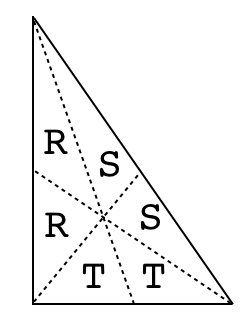
\includegraphics [scale=0.4] {centroid_tri.png} \end{center}

We draw lines from each vertex to the midpoint of the opposite side.  The three lines cross at a single point, the centroid.  (We looked at the proof of this in Ceva's Theorem).  It is easy to see that the areas of the small triangles with the same letter are equal.  

For example, both triangles $T$ have the same base (because we drew the median), and the same height.  For the same reason
\[ R + R + T = S + S + T \]
\[ R + R = S + S \]
That is
\[ R = S \]
As well
\[ R = S = T \]
The extension to $T$ follows because the problem is symmetrical.  

Now consider the median shown in red in the figure below and the altitude drawn to it.

\begin{center} 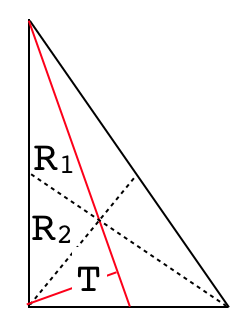
\includegraphics [scale=0.4] {centroid_tri2.png} \end{center}

Both the triangle labeled $T$ and the triangle formed from $R_1 + R_2$ have the same altitude as their height.  But the area of $R_1 + R_2$ together is twice that of $T$.  

Therefore the length of the base of $R_1 + R_2$ (along the median shown in red) must be twice that for the triangle labeled $T$.  That is, the centroid --- the point where the lines meet --- lies at $2/3$ of the distance from the vertex to the opposing side or $1/3$ of the way up from the bottom

Since we have a right triangle, then by similar triangles, both the $x$-coordinate and the $y$-coordinate of the centroid are at $1/3$.

We've seen this result produced by three different arguments in this book.  Once when looking at Ceva's Theorem geometrically, once using vectors, once by calculus in the chapter on average value, and now again here.  It is not only reassuring to find the same answer each time, but positively required.

 There is yet another proof that comes from Euler's construction of the three points on the same line:  orthocenter, centroid and circumcenter, and showing that the distance from centroid to orthocenter is twice that from centroid to circumcenter.  I'll put that into the Addendum.

\subsection*{centroid of the sphere's lamina}
The last part is the centroid of the half-circle.  Clearly, the average value of $x$ is zero by symmetry.  We need to compute the average value of $y$ \emph{over the whole area}.

\[ \bar{y} = \frac{\int_R y \ dA}{\int_R dA} \]

We don't actually need to compute the denominator.  It is just one-half the area of the circle or one-half $\pi R^2$.  

We'll do the integral of the numerator both ways, but first by polar coordinates.

We want
\[ \int_R y \ dA \]
Here $R$ stands for \emph{region}, but we want to use it below for \emph{radius} so let's suppress it.
\[ \int y \ dA \]

To get $y$ in radial coordinates I was tempted to write:
\[ y = R \sin \theta \]

but that is not correct!  I need a variable $r$ because $x$ and $y$ range over the entire area (this is a double integral, after all).
\[ y = r \sin \theta \]
So
\[ \iint y \ dA = \int_0^{\pi} \int_0^R r \sin \theta \ r \ dr \ d \theta \]
\[ = \int_0^{\pi} \int_0^R \sin \theta \ r^2 \ dr \ d \theta \]

The inner integral is
\[ \int_0^R \sin \theta \ r^2 \ dr \]
\[ = \sin \theta \ \frac{R^3}{3} \]

So the outer integral is
\[ \frac{R^3}{3} \int_0^{\pi} \sin \theta  \ d \theta \]
\[ \frac{R^3}{3} \ [ \ - \cos \theta \ \bigg |_0^{\pi} \ ] = \frac{2R^3}{3} \]

We remember to divide by $(1/2)\pi R^2$.

Multiplying by the inverse, we have then:
\[ \frac{2R^3}{3} \cdot \frac{2}{\pi R^2} = \frac{4R}{3 \pi} \]
which is exactly what we said before.

\subsection*{subtle error}

We want
\[ \int y \ dA \]
In Cartesian coordinates:
\[ = \int_{-R}^R \int y \ dy \ dx \]
What are the bounds on $y$?  It ranges from $0$ to $\sqrt{R^2 - x^2}$:
\[ = \int_{-R}^R \int_0^{\sqrt{R^2 - x^2}} \ y \ dy \ dx \]

Here I was tempted to substitute for $y$ in the integrand, and write
\[ = \int_{-R}^R \int_0^{\sqrt{R^2 - x^2}} \ \sqrt{R^2 - x^2} \ dy \ dx \]
but this is \emph{not correct}.

It is actually the same error as when I wanted to write $y = R \sin \theta$ above.  The thing is that $y$ as a bound is a constant (for that slice) and the substitution is OK.  It is not OK in the integrand, where $y$ is a variable.

The inner integral is just
\[ \int y \ dy = \frac{y^2}{2} \ \bigg |_0^{\sqrt{R^2 - x^2}} \]
\[ = \frac{R^2 - x^2}{2} \]
The outer integral is
\[ \int_{-R}^R \ \frac{R^2 - x^2}{2} \ dx \]
A simplification since both parts are even functions of $x$ 
\[ = 2 \int_0^R \ \frac{R^2 - x^2}{2} \ dx \]
\[ = 2 \ \frac{1}{2} \ [ \  R^2 x - \frac{x^3}{3} \ ] \ \bigg |_0^R \]
\[ = R^3 - \frac{R^3}{3} = \frac{2}{3}R^3 \]
as before.

\end{document}